\documentclass[12pt,fleqn, beamer]{beamer}


\xdefinecolor{lavendar}{rgb}{0.8,0.6,1}
\xdefinecolor{olive}{cmyk}{0.64,0,0.95,0.4}
%\xdefinecolor{olive}{cmyk}{1,0,0,0}
\xdefinecolor{mag}{cmyk}{0.1,1,0,0.2}
\xdefinecolor{lblue}{rgb}{0,0,1.5}
\xdefinecolor{lred}{rgb}{1,0,0}
\xdefinecolor{mine}{cmyk}{1,0,0.2,0}
\xdefinecolor{bluel}{cmyk}{0.1,0,0.9,0.4}

\usepackage{amsmath,amssymb,dsfont,mathrsfs}
\usepackage{tikz,pgflibraryplotmarks}
\usepackage{multimedia}
\usepackage{wasysym}
\usepackage{rotating}
\usepackage{algorithm,algorithmic}
\usepackage{graphicx} % more modern
\usepackage{subfigure}
\usepackage{booktabs}

\usepackage{pgfplots}
\usepackage{verbatim}

\usepackage{setspace}
\newlength\iwidth
\newlength\iheight

\newcommand\makebeamertitle{\frame{\maketitle}}%
\graphicspath{{./images/}}
\setbeamertemplate{navigation symbols}{}
\addtobeamertemplate{navigation symbols}{}{%
    \usebeamerfont{footline}%
    \usebeamercolor[fg]{footline}%
	\insertshorttitle
    \;--
    \insertframenumber
}

\newcommand{\sectionstart}{
	\only<beamer>{
 	\begin{frame}% (fold)
 		\begin{centering}\Huge \insertsection \par\end{centering}
 	\end{frame}% frame the_application (end)
	}
 }


% make bibliography entries smaller
\usepackage{natbib}
\setbeamertemplate{bibliography item}{[\theenumiv]}
\renewcommand\bibfont{\scriptsize}
\setbeamertemplate{frametitle continuation}[from second]
\newcommand{\tcr}{\textcolor{red}}
\newcommand{\tcrd}{\textcolor{red}}
\newcommand{\tcb}{\textcolor{bluel}}
\newcommand{\tcm}{\textcolor{mag}}
\newcommand{\tcg}{\textcolor{olive}}

\newcommand{\R}{\mathbb{R}}
\newcommand{\C}{\mathbb{C}}

% bold lower-case for vectors
\newcommand{\bfa}{{\bf a}}
\newcommand{\bfb}{{\bf b}}
\newcommand{\bfc}{{\bf c}}
\newcommand{\bfs}{{\bf s}}
\newcommand{\bfm}{{\bf m}}
\newcommand{\bfd}{{\bf d}}
\newcommand{\bfe}{{\bf e}}
\newcommand{\bfu}{{\bf u}}
\newcommand{\bfy}{{\bf y}}
\newcommand{\bfx}{{\bf x}}
\newcommand{\bfh}{{\bf h}}
\newcommand{\bfw}{{\bf w}}
\newcommand{\bfv}{{\bf v}}
\newcommand{\bfr}{{\bf r}}
\newcommand{\bfz}{{\bf z}}
\newcommand{\bff}{{\bf f}}
\newcommand{\bfp}{{\bf p}}


% bold upper-case for linear operators
\newcommand{\bfA}{{\bf A}}
\newcommand{\bfB}{{\bf B}}
\newcommand{\bfZ}{{\bf Z}}
\newcommand{\bfM}{{\bf M}}
\newcommand{\bfC}{{\bf C}}
\newcommand{\bfD}{{\bf D}}
\newcommand{\bfQ}{{\bf Q}}
\newcommand{\bfJ}{{\bf J}}
\newcommand{\bfG}{{\bf G}}
\newcommand{\bfI}{{\bf I}}
\newcommand{\bfP}{{\bf P}}
\newcommand{\bfK}{{\bf K}}
\newcommand{\bfY}{{\bf Y}}
\newcommand{\bfW}{{\bf W}}
\newcommand{\bfR}{{\bf R}}
\newcommand{\bfL}{{\bf L}}
\newcommand{\bfF}{{\bf F}}
\newcommand{\bfT}{{\bf T}}
\newcommand{\bfS}{{\bf S}}
\newcommand{\bfX}{{\bf X}}
\newcommand{\bfU}{{\bf U}}
\newcommand{\bfV}{{\bf V}}
\newcommand{\bfH}{{\bf H}}

\newcommand{\diag}{\rm diag}

\newcommand{\calF}{\mathcal{F}}
\newcommand{\calN}{\mathcal{N}}
\newcommand{\calT}{\mathcal{T}}
\newcommand{\calX}{\mathcal{X}}




\newcommand{\hf}{{\frac 12}}
\newcommand{\bftheta}{{\boldsymbol \theta}}
\newcommand{\bfmu}{{\boldsymbol \mu}}
\newcommand{\bfxi}{{\boldsymbol \xi}}

\newcommand{\bfLambda}{{\boldsymbol \Lambda}}
\newcommand{\bflambda}{{\boldsymbol \lambda}}
\newcommand{\bfSigma}{{\boldsymbol \Sigma}}
\newcommand{\bfepsilon}{{\boldsymbol \epsilon}}

\newcommand{\E}{\vec E}
\newcommand{\B}{\vec B}

\newcommand{\vu}{  {\vec {\bf u}}}

\newcommand{\grad}{  {\vec {\bf \nabla}}}

\newcommand{\lfrownie}{\textcolor{red}{\large{\frownie}}}
\newcommand{\lsmiley}{\textcolor{green}{\large{\smiley}}}

\newcommand{\curl}{\ensuremath{\nabla\times\,}}
\renewcommand{\div}{\nabla\cdot\,}
\newcommand{\divh}{\nabla_h\cdot\,}
\renewcommand{\grad}{\ensuremath{\nabla}}

\DeclareMathOperator*{\argmin}{arg\,min}

\usepackage{animate}

\title[OC]{Optimal Control}
\subtitle{Numerical Methods for Deep Learning}
\date{}
\begin{document}

\makebeamertitle

\begin{frame}
	\frametitle{Learning Objective: Optimal Control}
	
	In this module we discuss optimal control methods for ResNet training 
	
	\bigskip
	
	Learning tasks:
	\begin{itemize}
		\item regression
		\item segmentation
		\item classification
	\end{itemize}
	
	\bigskip
	
	Concepts from optimal control
	\begin{itemize}
		\item optimize-then-discretize vs. discretize-then-optimize \cite{Onken2020DO}
		\item backpropagation vs. adjoint equations
	\end{itemize}
\end{frame}

\section{Optimization Problem} % (fold)
\label{sec:optimization_problem}
\begin{frame}[fragile]\frametitle{Residual Network as a Path Planning Problem}

Change in notation: Moving forward it is more convenient to define $\bfY \in \R^{n_f \times n}$ (transpose data matrix) and $\bfC \in \R^{n_c \times n}$. 

$$ \partial_t{\bfY}(t) = \sigma(\bfK(t) \bfY(t)  + b(t)) \quad \bfY(0) = \bfY_0 $$

The goal is to plan a path such that the transformed features, $\bfY(T)$, can be linearly separated.


\begin{center}
	\begin{tabular}{cc}
		\includegraphics[width=45mm]{Circle-train} & 
		\invisible<beamer|1>{\includegraphics[width=45mm]{Circle-proptrain} }\\
		input features, $\bfY(0)$ & \invisible<beamer|1>{transformed features $\bfY(T)$}
	\end{tabular}
\end{center}
\only<beamer|2>{}
\end{frame}

	\begin{frame}
		\frametitle{Example: The Adjoint Equation}
		
		Simplified learning problem: one example $(\bfy_0, \bfc)$, no weights for classifier, no regularizer, $\bfy(0,\bftheta) = \bfy_0$
		\begin{equation*}
			\min_{\bftheta} {\rm loss}(\bfy(1,\bftheta), \bfc) \; \text{ with } \; \partial_t \bfy(t,\bftheta) = f(\bfy(t),\bftheta(t)).
		\end{equation*}
		\pause
		Use adjoint method to compute gradient of objective w.r.t. $\bftheta$
		\begin{equation*}
			\frac{\partial {\rm loss}}{\partial \bftheta}(t) = \left(\frac{\partial f}{\partial \bftheta}({\bfy(t,\bftheta)}, \bftheta(t))\right)^\top \bfz(t)
		\end{equation*}
		where $\bfz$ satisfies the adjoint method ($-\partial_t \leadsto$ backward in time)
		\begin{align*}
			-\partial_t \bfz(t,\bftheta) = \left(\frac{\partial f}{\partial \bfy} ({\bfy(t,\bftheta)},\bftheta(t))\right)^\top \bfz(t), \\
			\bfz(1,\bftheta)= \frac{\partial {\rm loss}}{\partial \bfy} ({\bfy(1,\bftheta)}, \bfc).
		\end{align*}
		\pause
	\begin{center}
		\textbf{note: $\bfy(t)$ needed to solve adjoint equation (memory!)}
	\end{center}
	
	% \begin{columns}
% 		\column{.5\textwidth}
% 		\begin{thebibliography}{1}
% 		\scriptsize
% 		\bibitem{ResNN} G. A. Bliss\\
% 		\newblock{\sl The use of adjoint systems in the problem of differential corrections for trajectories}.
% 		\newblock{JUS Artillery, 51:296–311, 1919}
% 		\end{thebibliography}
%
% 		\column{.5\textwidth}
% 		\begin{thebibliography}{1}
% 		\scriptsize
% 		\bibitem{ResNN} D.E. Rumelhart, G.E. Hinton, R.J. Williams\\
% 		\newblock{\sl Learning representations by back-propagating errors}.
% 		\newblock{Nature, 533–536, 1986.}
% 		\end{thebibliography}
% 	\end{columns}
	\end{frame}
	% \end{document}
	\begin{frame}
		\frametitle{ Diff$\rightarrow$Disc vs. Disc$\rightarrow$Diff  \cite{Onken2020DO}}
		\begin{equation*}
			\min_{\bftheta} {\rm loss}(\bfY(1,\bftheta), \bfC) \; \text{ with } \; \partial_t \bfY(t,\bftheta) = f(\bfY(t),\bftheta(t)).
		\end{equation*}
	 	
		\pause
			\textbf{First-Differentiate-then-Discretize ( Diff$\rightarrow$Disc)}
			\begin{itemize}
				\item Keep $\bftheta, \bfY$ continuous in time
				\item Euler-Lagrange-Equations $\leadsto$ adjoint equation ($\approx$ backprop)
				\item flexible choice of ODE solver in forward and adjoint
				\item gradients only useful if fwd and adjoint solved well
				
				\item use optimization to obtain discrete solution of ELE
			\end{itemize}
			\pause
			\bigskip
			
			{\textbf{First-Discretize-then-Differentiate (Disc$\rightarrow$Diff)}}
			\begin{itemize}
				\item Discretize $\bftheta, \bfY$ in time (could use different grids)
				\item Differentiate objective (e.g., use automatic differentiation)
				\item gradients related to adjoints but no choice of solver
				\item gradients useful even if discretization is inaccurate 
				\item use nonlinear optimization tools to approximate minimizer
			\end{itemize}
		
		% 		\begin{columns}
		% 			\column{.33\textwidth}
		%
		% 			\begin{thebibliography}{1}
		% 			\scriptsize
		% 			\bibitem{2013Multigrid} MD Gunzburger
		% 			\newblock{\sl Perspectives in flow control and optimization}.
		% 			\newblock{SIAM,  2013.}
		% 			\end{thebibliography}
		%
		% 			\column{.30\textwidth}
		% 			\begin{thebibliography}{1}
		% 			\scriptsize
		% 			\bibitem{2013Multigrid2} TQ Chen et al.,
		% 			\newblock{\sl Neural Ordinary Differential Equations}.
		% 			\newblock{NeurIPS, 2018.}
		% 			\end{thebibliography}
		%
		% 			\column{.36\textwidth}
		% 			\begin{thebibliography}{1}
		% 			\scriptsize
		% 			\bibitem{2013Multigrid2} A Gholami, K Keutzer, G Biros
		% 			\newblock{\sl ANODE: Unconditionally Accurate Memory-Efficient Gradients for Neural ODEs}.
		% 			\newblock{arXiv:1902.10298}
		% 		\end{thebibliography}
		% \end{columns}
	\end{frame}
	

	\begin{frame}
			\frametitle{Example: Gradient Test Disc$\rightarrow$Diff}
			
			Goal: Find weights of neural network $F(\bfu,\theta)$ such that
			\begin{equation*}
				\partial_t \bfu = F(\bfu,\theta),\quad \bfu(0) = \bfu_0
			\end{equation*}
			fits true ODE at $0< t_1 < t_2 < \cdots < t_n \leq 1.5$; details Sec. 8 from paper below.
			
			\bigskip
			
			Question: How does accuracy of ODE solvers impact the quality of gradient?
			
			\begin{center}
				\scriptsize
				\iwidth=.25\textwidth
				\iheight=.25\textwidth
				\begin{tabular}{rrr}
					% This file was created by matlab2tikz.
% Minimal pgfplots version: 1.3
%
%The latest updates can be retrieved from
%  http://www.mathworks.com/matlabcentral/fileexchange/22022-matlab2tikz
%where you can also make suggestions and rate matlab2tikz.
%
\definecolor{mycolor1}{rgb}{0.00000,0.44700,0.74100}%
\definecolor{mycolor2}{rgb}{0.85000,0.32500,0.09800}%
%
\begin{tikzpicture}

\begin{axis}[%
width=0.95092\iwidth,
height=\iheight,
at={(0\iwidth,0\iheight)},
scale only axis,
xmode=log,
xmin=9e-07,
xmax=0.5,
xminorticks=true,
ymode=log,
ymin=1e-7,
ymax=1e3,
yminorticks=true,
legend style={at={(0.97,0.03)},anchor=south east,legend cell align=left,align=left,draw=white!15!black}
]
\addplot [color=mycolor1,solid, ultra thick]
  table[row sep=crcr]{%
0.5 3863.578046107106\\
0.25    4664.453710787793\\
0.125   4429.827191810487\\
0.0625  3737.079020947542\\
0.03125 2193.7491856822994\\
0.015625    220.60886142236677\\
0.0078125   87.43529688756644\\
0.00390625  40.340004245386126\\
0.001953125 19.490721069911615\\
0.0009765625    9.592178761714422\\
0.00048828125   4.759688785757135\\
0.000244140625  2.3709710814766822\\
0.0001220703125 1.183294981422705\\
6.103515625e-5  0.5911032866983987\\
3.0517578125e-5 0.29541601965752307\\
1.52587890625e-5    0.1476741571857474\\
7.62939453125e-6    0.0738286220844202\\
3.814697265625e-6   0.03691219774464116\\
1.9073486328125e-6  0.01845557065189496\\
9.5367431640625e-7  0.009227653285279303\\
};
\addlegendentry{E0};

\addplot [color=mycolor2,solid, ultra thick]
  table[row sep=crcr]{%
0.5 974.3007134763934\\
0.25    2245.5143309960436\\
0.125   3220.357501914613\\
0.0625  3132.344175999605\\
0.03125 1891.3817632083308\\
0.015625    69.42515018538242\\
0.0078125   11.843441269074262\\
0.00390625  2.5440764361400383\\
0.001953125 0.592757165288571\\
0.0009765625    0.14319680940289992\\
0.00048828125   0.03519780960137364\\
0.000244140625  0.008725593398801745\\
0.0001220703125 0.002172237383764708\\
6.103515625e-5  0.0005419146789286122\\
3.0517578125e-5 0.00013533364778800516\\
1.52587890625e-5    3.381418087985977e-5\\
7.62939453125e-6    8.450581986438332e-6\\
3.814697265625e-6   2.1119934242794236e-6\\
1.9073486328125e-6  5.277762865178726e-7\\
9.5367431640625e-7  1.3184747508186712e-7\\
};
\addlegendentry{E1};

\end{axis}
\end{tikzpicture}%
				&
					\invisible<beamer|1>{% This file was created by matlab2tikz.
% Minimal pgfplots version: 1.3
%
%The latest updates can be retrieved from
%  http://www.mathworks.com/matlabcentral/fileexchange/22022-matlab2tikz
%where you can also make suggestions and rate matlab2tikz.
%
\definecolor{mycolor1}{rgb}{0.00000,0.44700,0.74100}%
\definecolor{mycolor2}{rgb}{0.85000,0.32500,0.09800}%
%
\begin{tikzpicture}

\begin{axis}[%
width=0.95092\iwidth,
height=\iheight,
at={(0\iwidth,0\iheight)},
scale only axis,
xmode=log,
xmin=9e-07,
xmax=0.5,
xminorticks=true,
ymode=log,
ymin=1e-7,
ymax=1e3,
yminorticks=true,
legend style={at={(0.97,0.03)},anchor=south east,legend cell align=left,align=left,draw=white!15!black}
]
\addplot [color=mycolor1,solid, ultra thick]
  table[row sep=crcr]{%
0.5 3863.715338573592\\
0.25    4528.7476490279005\\
0.125   4428.7827534967355\\
0.0625  3736.8581654499076\\
0.03125 2200.034318131339\\
0.015625    220.59515728576798\\
0.0078125   87.43194832745644\\
0.00390625  40.34030494666695\\
0.001953125 19.49167226199529\\
0.0009765625    9.592862778530844\\
0.00048828125   4.760076444066726\\
0.000244140625  2.371175024318063\\
0.0001220703125 1.183399296433663\\
6.103515625e-5  0.5911560057288625\\
3.0517578125e-5 0.2954425164393797\\
1.52587890625e-5    0.14768743949912277\\
7.62939453125e-6    0.07383527167121429\\
3.814697265625e-6   0.036915524641472075\\
1.9073486328125e-6  0.01845723462542992\\
9.5367431640625e-7  0.009228485400626596\\
};
\addlegendentry{E0};

\addplot [color=mycolor2,solid, ultra thick]
  table[row sep=crcr]{%
0.5 978.3728900773576\\
0.25    2271.1795349544304\\
0.125   3239.3018205145872\\
0.0625  3132.299270920899\\
0.03125 1937.521654162317\\
0.015625    69.08634590910506\\
0.0078125   11.646004490124895\\
0.00390625  2.418250284074851\\
0.001953125 0.5255570965649277\\
0.0009765625    0.1127457963998868\\
0.00048828125   0.02176174179637247\\
0.000244140625  0.002565885070121343\\
0.0001220703125 0.0007589798273623938\\
6.103515625e-5  0.000885801415703269\\
3.0517578125e-5 0.0005689862071977525\\
1.52587890625e-5    0.0003159547535952212\\
7.62939453125e-6    0.00016583543887420393\\
3.814697265625e-6   8.488132361413742e-5\\
1.9073486328125e-6  4.293145015924968e-5\\
9.5367431640625e-7  2.1588408525249556e-5\\
};
\addlegendentry{E1};

\end{axis}
\end{tikzpicture}%}
				&
					\invisible<beamer|-2>{% This file was created by matlab2tikz.
% Minimal pgfplots version: 1.3
%
%The latest updates can be retrieved from
%  http://www.mathworks.com/matlabcentral/fileexchange/22022-matlab2tikz
%where you can also make suggestions and rate matlab2tikz.
%
\definecolor{mycolor1}{rgb}{0.00000,0.44700,0.74100}%
\definecolor{mycolor2}{rgb}{0.85000,0.32500,0.09800}%
%
\begin{tikzpicture}

\begin{axis}[%
width=0.95092\iwidth,
height=\iheight,
at={(0\iwidth,0\iheight)},
scale only axis,
xmode=log,
xmin=1e-07,
xmax=1,
xminorticks=true,
ymode=log,
ymin=1e-7,
ymax=1e3,
yminorticks=true,
legend style={at={(0.97,0.03)},anchor=south east,legend cell align=left,align=left,draw=white!15!black}
]
\addplot [color=mycolor1,solid, ultra thick]
  table[row sep=crcr]{%
0.5 3863.715338573592\\
0.25    4528.7476490279005\\
0.125   4428.7827534967355\\
0.0625  3736.8581654499076\\
0.03125 2200.034318131339\\
0.015625    220.59515728576798\\
0.0078125   87.43194832745644\\
0.00390625  40.34030494666695\\
0.001953125 19.49167226199529\\
0.0009765625    9.592862778530844\\
0.00048828125   4.760076444066726\\
0.000244140625  2.371175024318063\\
0.0001220703125 1.183399296433663\\
6.103515625e-5  0.5911560057288625\\
3.0517578125e-5 0.2954425164393797\\
1.52587890625e-5    0.14768743949912277\\
7.62939453125e-6    0.07383527167121429\\
3.814697265625e-6   0.036915524641472075\\
1.9073486328125e-6  0.01845723462542992\\
9.5367431640625e-7  0.009228485400626596\\
};
\addlegendentry{E0};

\addplot [color=mycolor2,solid, ultra thick]
  table[row sep=crcr]{%
0.5 1105.9162181005531\\
0.25    2001.0474056718367\\
0.125   2967.3395679928703\\
0.0625  2894.6767600054736\\
0.03125 1791.905644041919\\
0.015625    67.53447526843416\\
0.0078125   11.535795928967019\\
0.00390625  2.4792596176008743\\
0.001953125 0.577791181428843\\
0.0009765625    0.13959757954475904\\
0.00048828125   0.0343151250601057\\
0.000244140625  0.008507035579179423\\
0.0001220703125 0.0021178686123275448\\
6.103515625e-5  0.0005283606602033419\\
3.0517578125e-5 0.00013195215128825044\\
1.52587890625e-5    3.2970804750898086e-5\\
7.62939453125e-6    8.240548345722631e-6\\
3.814697265625e-6   2.0598687230505286e-6\\
1.9073486328125e-6  5.149332140200191e-7\\
9.5367431640625e-7  1.28729905710806e-7\\
};
\addlegendentry{E1};

\end{axis}
\end{tikzpicture}%}\\
					 $\epsilon_{\rm rel}=10^{-7}, \epsilon_{\rm abs}=10^{-9}$
					&
					 \invisible<beamer|1>{$\epsilon_{\rm rel}=10^{-2}, \epsilon_{\rm abs}=10^{-2}$}
					 &
					 \invisible<beamer|-2>{Disc$\rightarrow$Diff, rk4, $n_t=30$}
				\end{tabular}
			\end{center}
	
	\end{frame}
	
	\begin{frame}
		\frametitle{Example: Training Disc$\rightarrow$Diff}
		
		\begin{columns}
			
		   \column{.5\textwidth}
		   \begin{center}
			   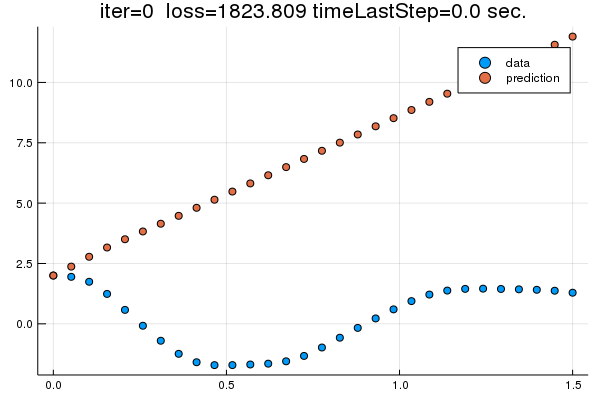
\includegraphics[width=1.\textwidth]{node/node-tol-1e-2/NODE-f64-reltol-1e-2-iter-0}
			Neural ODE, $\epsilon_{\rm rel}=10^{-7}, \epsilon_{\rm abs}=10^{-9}$\\
		   \end{center}
		   % \column{.5\textwidth}
		   %   \animategraphics[autoplay, width=1.\textwidth]{3}{\Fimage{DeepLearning/numerics/node/node-tol-1e-2/NODE-f64-reltol-1e-2-iter-}}{1}{2}
		   \column{.5\textwidth}
		   \begin{center}			   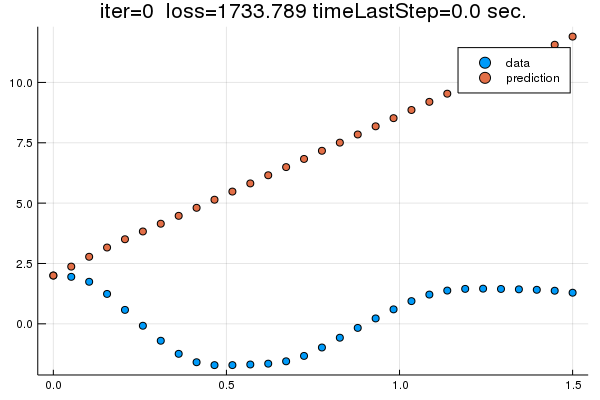
\includegraphics[width=1.\textwidth]{node/node-rk4/rk4-iter-0}
			Disc$\rightarrow$Diff, RK4, 30 steps
		   \end{center}
		\end{columns}
		
		\bigskip
		
		Training: ADAM with default setting, same initialization
	\end{frame}
	
	
	\begin{frame}
		\frametitle{}
		\begin{columns}
			
		   \column{.5\textwidth}
		   \begin{center}
		     \animategraphics[autoplay, width=1.\textwidth,every=5]{3}{node/node-tol-1e-7/NODE-f64-reltol-1e-7-iter-}{0}{300}
			Neural ODE, $\epsilon_{\rm rel}=10^{-7}, \epsilon_{\rm abs}=10^{-9}$\\
		   \end{center}
		   % \column{.5\textwidth}
		   %   \animategraphics[autoplay, width=1.\textwidth]{3}{\Fimage{DeepLearning/numerics/node/node-tol-1e-2/NODE-f64-reltol-1e-2-iter-}}{1}{2}
		   \column{.5\textwidth}
		   \begin{center}
			\animategraphics[autoplay, width=1.\textwidth,every=5]{3}{node/node-rk4/rk4-iter-}{0}{300}
			Disc$\rightarrow$Diff, RK4, 30 steps
		   \end{center}
		\end{columns}
		\bigskip
		
		Training: ADAM with default setting, same initialization
	\end{frame}
	% \end{document}
	
	\begin{frame}
		\frametitle{}
		\begin{columns}
			
		   \column{.5\textwidth}
		   \begin{center}
		     \animategraphics[autoplay, width=1.\textwidth,every=5]{3}{node/node-tol-1e-2/NODE-f64-reltol-1e-2-iter-}{0}{300}
			Neural ODE, { $\epsilon_{\rm rel}=10^{-2}, \epsilon_{\rm abs}=10^{-2}$}\\
		   \end{center}
		   % \column{.5\textwidth}
		   %   \animategraphics[autoplay, width=1.\textwidth]{3}{\Fimage{DeepLearning/numerics/node/node-tol-1e-2/NODE-f64-reltol-1e-2-iter-}}{1}{2}
		   \column{.5\textwidth}
		   \begin{center}
			\animategraphics[autoplay, width=1.\textwidth,every=5]{3}{node/node-rk4/rk4-iter-}{0}{300}
			Disc$\rightarrow$Diff, RK4, 30 steps
		   \end{center}
		\end{columns}
		\bigskip
		
		Training: ADAM with default setting, same initialization
	\end{frame}
	
	
	
\begin{frame}\frametitle{Residual Network - Forward Propagation}

Idea: Obtain forward propagation by discretizing the ODE

$$ \partial_t{\bfY} = \sigma( \bfK\bfY + b) \quad \bfY(0) = \bfY_0 $$

\bigskip
\pause

Example: Use forward Euler method
\begin{eqnarray*}
\bfY_{j+1} = \bfY_j + h \sigma( \bfK_j\bfY_j + b_j)
\end{eqnarray*}
Here: $\bfY_j$ is called the \emph{state}, $\bfK_j, b_j$ are \emph{controls}, and $h>0$ is time step size.

\bigskip
\pause

More general forward propagation
\begin{eqnarray*}
\bfY_{j+1} =  \bfP_j \bfY_j + h \sigma(\bfK_j\bfY_j  + b_j), \qquad \bfP_j \text{ fixed.}
\end{eqnarray*}
Allows for changing resolution and width (and classical neural networks).


\end{frame}
% section optimization_problem (end)

\section{Computing Derivatives} % (fold)
\begin{frame}\frametitle{Residual Network - Optimization Problem}


Note: Only final state used in loss
$$ \min_{\bfW, \bfK_{0,\ldots,N-1},b_{0,\ldots,N-1}}E\left(
\bfW \bfY_N(\bfK_{0,\ldots,N-1},b_{0,\ldots,N-1}),\bfC^{\rm obs}\right) $$

\bigskip
\pause

Need to differentiate
\begin{itemize}
\item $E$ w.r.t $\bfW$

\item ${\cal S}$ w.r.t $\bfY_N$

\item $\bfY_N$ w.r.t control variables ($\bfK_{0,\ldots,N-1},b_{0,\ldots,N-1}$)
\end{itemize}

\bigskip
\pause

Having these, apply chain rule to get, e.g.,
$$
\grad_{\bfK_j} E =  \left(\bfJ_{\bfK_j} {\bfY_N}\right)^{\top} \grad_{\bfY_N} E
$$

How? Adjoint method~\cite{bliss1919,BorzSchulz2012} (more general than back propagation~\cite{Rumelhart1986})
\end{frame}


\begin{frame}\frametitle{Computing Derivatives - Sensitivity Equation}
Idea: Differentiate the forward propagation (forward Euler) with respect to $\bfK_i$ for fixed  $0\leq i \leq N$. Note that
$$
	\bfJ_{\bfK_i} \bfY_j = 0, \quad \text{ for } \quad j\leq i. 
$$

\smallskip
\pause

Next, note that 
$$
\bfJ_{\bfK_j} \bfY_{i+1} = h {\rm diag}(\sigma'( \bfK_i \bfY_i + b_i))
(  \bfY_i^\top \otimes \bfI)
$$

\smallskip
\pause

Continuing like this, gives for the final state:
\begin{eqnarray*}
\bfJ_{\bfK_i}\bfY_{N} & =& \bfP_{N-1}  \bfJ_{\bfK_i}\bfY_{N-1}  \\
	&  +& h {\rm diag}(\sigma'( \cdots)) \left( ( \bfI \otimes \bfK_{N-1}) \bfJ_{\bfK_i}\bfY_{N-1}\right) 
\end{eqnarray*}
\smallskip
\pause
Next: Write this as a block triangular {\bf linear} system.
\end{frame}


\begin{frame}\frametitle{Computing Derivatives - Sensitivity Equations}

Block triangular {\bf linear} system for the gradients
{\small
\begin{eqnarray*}
\begin{pmatrix}
\bfI              &                &                &          &       \\
-\bfT_{i+1}    &   \bfI       &                &          &       \\
                    & \ddots    &  \ddots    &          &      \\
                    &     &      &          &      \\
                    &     &        &   -\bfT_{N-1}       & \bfI
                    \end{pmatrix}
                    \begin{pmatrix}
                    \bfJ_{\bfK_i}\bfY_{i+1} \\    \\   \\ \\   \bfJ_{\bfK_i}\bfY_{N}
                    \end{pmatrix} =
                    \begin{pmatrix}
                    \bfR_i \\  0\\  \vdots \\ \\   0
                    \end{pmatrix}
\end{eqnarray*}}


$$\bfT_j = \bfP_j + h {\rm diag}(\sigma'( \bfK_j \bfY_j+ b_j))
(\bfI \otimes \bfK_j) $$

and 

$$ \bfR_i = h {\rm diag}(\sigma'(\bfK_i \bfY_i  + b_i)) ( \bfY_i^\top \otimes \bfI). $$


\end{frame}



\begin{frame}\frametitle{Computing Derivatives - Sensitivity Equation}

Block triangular {\bf linear} system for the gradients
{\small
\begin{eqnarray*}
	\underbrace{
\begin{pmatrix}
\bfI              &                &                &          &       \\
-\bfT_{i+1}    &   \bfI       &                &          &       \\
                    & \ddots    &  \ddots    &          &      \\
                    &     &      &          &      \\
                    &     &        &   -\bfT_{N-1}       & \bfI
                    \end{pmatrix}}_{=\bfT}
					\underbrace{
                    \begin{pmatrix}
                    \bfJ_{\bfK_i}\bfY_{i+1} \\    \\   \\ \\   \bfJ_{\bfK_i}\bfY_{N}
                    \end{pmatrix}}_{= {\bfJ_{\bfK_i} \bfY}} =
					\underbrace{
                    \begin{pmatrix}
                    \bfR_i \\  0\\  \vdots \\ \\    0
                    \end{pmatrix}}_{=\bfR}
\end{eqnarray*}}

To compute matrix-vector product $(\bfJ_{\bfK_i}\bfY_{N})\, \bfv$
\begin{itemize}
\item Multiply $\bfR\, \bfv$
\item Solve (forward propagate) $\bfT\, \bfJ_{\bfK_i}\bfY = \bfR\, \bfv$
\item Extract the last time step
\end{itemize}

\end{frame}

\section{Summary} % (fold)
\label{sec:numerical_optimization}
\begin{frame}[fragile]\frametitle{$\Sigma$: Optimal Control}

Biggest question: Continuous vs. discrete
$$ \min_{\bfW, \bfY(T,\bftheta)}E\left(
\bfW \bfY(T,\bftheta),\bfC^{\rm obs}\right) 
\; \text{ vs. }\;
 \min_{\bfW, \bfY_N(\bftheta)}E\left(
\bfW \bfY_N(\bftheta),\bfC^{\rm obs}\right) $$

Continuous model
\begin{itemize}
	\item[+] can help initialization (easy to add layers)
	\item[+] simplifies analysis and insight
	\item[+] inspires better architectures (discrete!)
	\item[-] high accuracy needs high computational costs
	\item[-] meaningful (dynamics not derived from 1st principles?)
\end{itemize}

Discrete model
\begin{itemize}
	\item[+] back propagation easier than solving adjoint equations
	\item[+] accurate gradients even for large time steps
	\item[+] computationally more efficient
	\item[-] may 'overfit' on a given discretization
	\item[-] need careful discretization
\end{itemize}

\end{frame}


% \begin{frame}\frametitle{The Sensitivity Equation}
%
%
% Symbolically
%
% $$ \bfJ_{\bfK_i}\bfY_{N}  = \bfQ \bfT^{-1}  \bfR  $$
% where
% $$\bfQ = [0,\ldots,\bfI]. $$
%
%
% \bigskip
%
% The transpose
%
% $$ \left(\bfJ_{\bfK_i}\bfY_{N}\right)^{\top} =  \bfR^{\top} \bfT^{-T} \bfQ^{\top} $$
%
%
% \end{frame}
%
% \begin{frame}\frametitle{The Sensitivity Equation}
%
% $$ \left(\grad_{\bfK_i}\bfY_{N}\right)^{\top} =  \bfR^{\top} \bfT^{-T} \bfQ^{\top} $$
%
%
% {\small
% \begin{eqnarray*}
% \begin{pmatrix} \bfR_i^{\top}  &   0   &  \hdots     &   & 0 \end{pmatrix}
% \begin{pmatrix}
% \bfI              &  -\bfT_{i+1}^{\top}  &                &          &       \\
%                     &   \bfI       &     -\bfT_{i+2}^{\top}           &          &       \\
%                     &     &  \ddots    &    \ddots      &      \\
%                     &     &      &    \bfI      &  -\bfT_{N}    \\
%                     &     &        &          & \bfI
%                     \end{pmatrix}^{-1}
%   \begin{pmatrix} 0 \\    \\   \vdots  \\    \\  \bfI \end{pmatrix}
% \end{eqnarray*}
% }
%
%
%
% To multiply by the transpose
% \begin{itemize}
% \item Initialize with last step
% \item {\bf solve backward} in time
% \item Extract the first step and multiply by $\bfR_i^{\top} $
% \end{itemize}
%
% \end{frame}
%
% \begin{frame}\frametitle{More about the sensitivity equation}
%
% To compute $({\bfJ_{\bfK_i}}\bfY_N)^{\top} $ for all $i$'s note that the same quantities
% are recomputed. Can be evaluated in ${\cal O}(N)$ steps
%
% \bigskip
%
% For gradient based method the transpose is sufficient
%
% \bigskip
%
% Newton based methods require both forward sensitivities and adjoint.
%
%
% \end{frame}


\begin{frame}[allowframebreaks]
	\frametitle{References}
\bibliographystyle{abbrv}
\bibliography{NumDNN}

\end{frame}
\end{document}
















